\begin{figure*}[t]
\begin{center}
    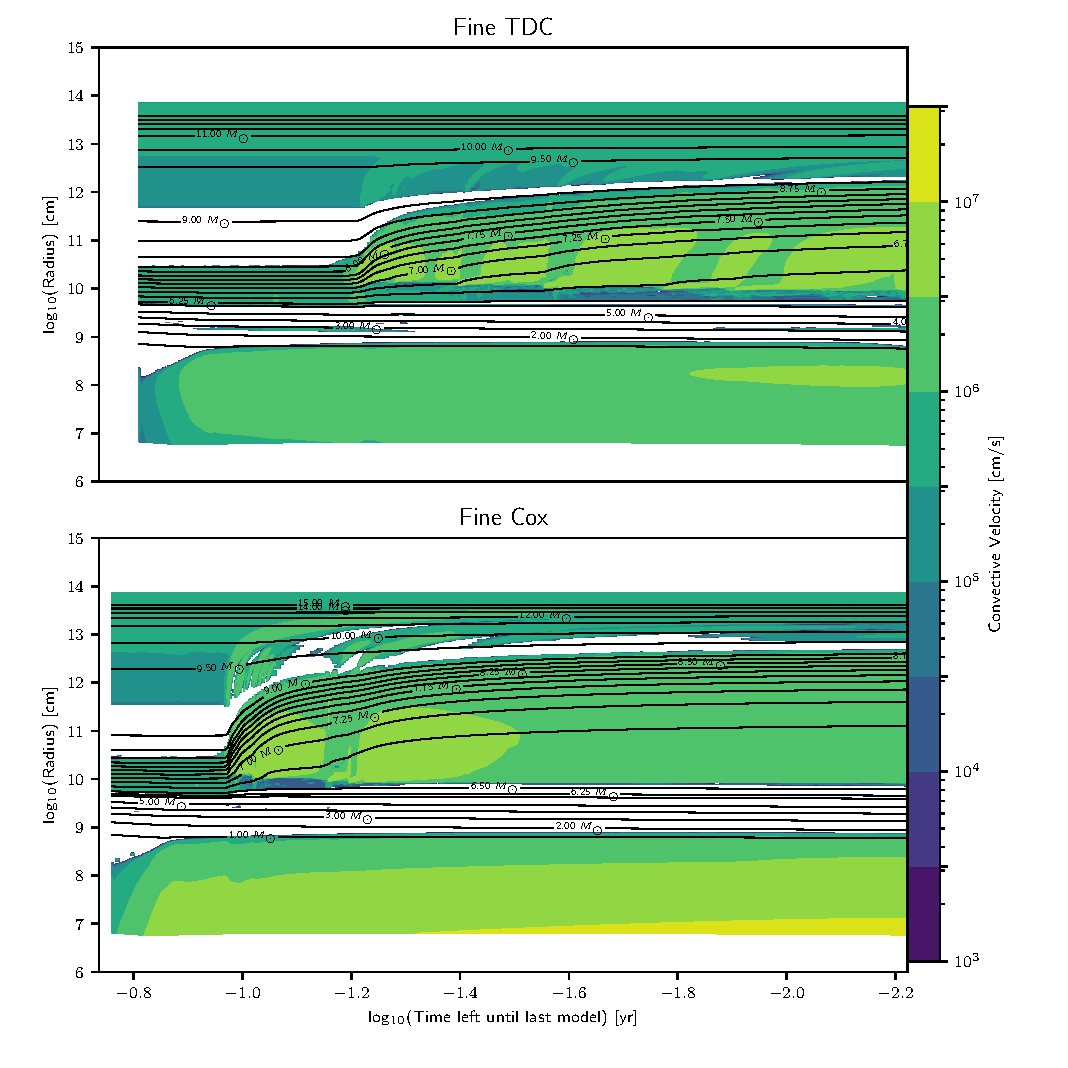
\includegraphics[width=0.9\linewidth]{Figures/KHD_Compare_Mix.pdf}
    \caption{Kippenhahn diagrams of radius (logarithmic) by time until core collapse, comparing an \gls{MLT} (lower) and \gls{TDC} (upper) run using short timestepping, focusing on a shell merger. Colour pertains to convective velocity.}
    \label{fig:KHD_Compare_Mix}
\end{center}
\end{figure*}

%%%%%%
% \begin{figure*}[t]
% \centering
% \begin{subfigure}{0.6\textwidth}
%     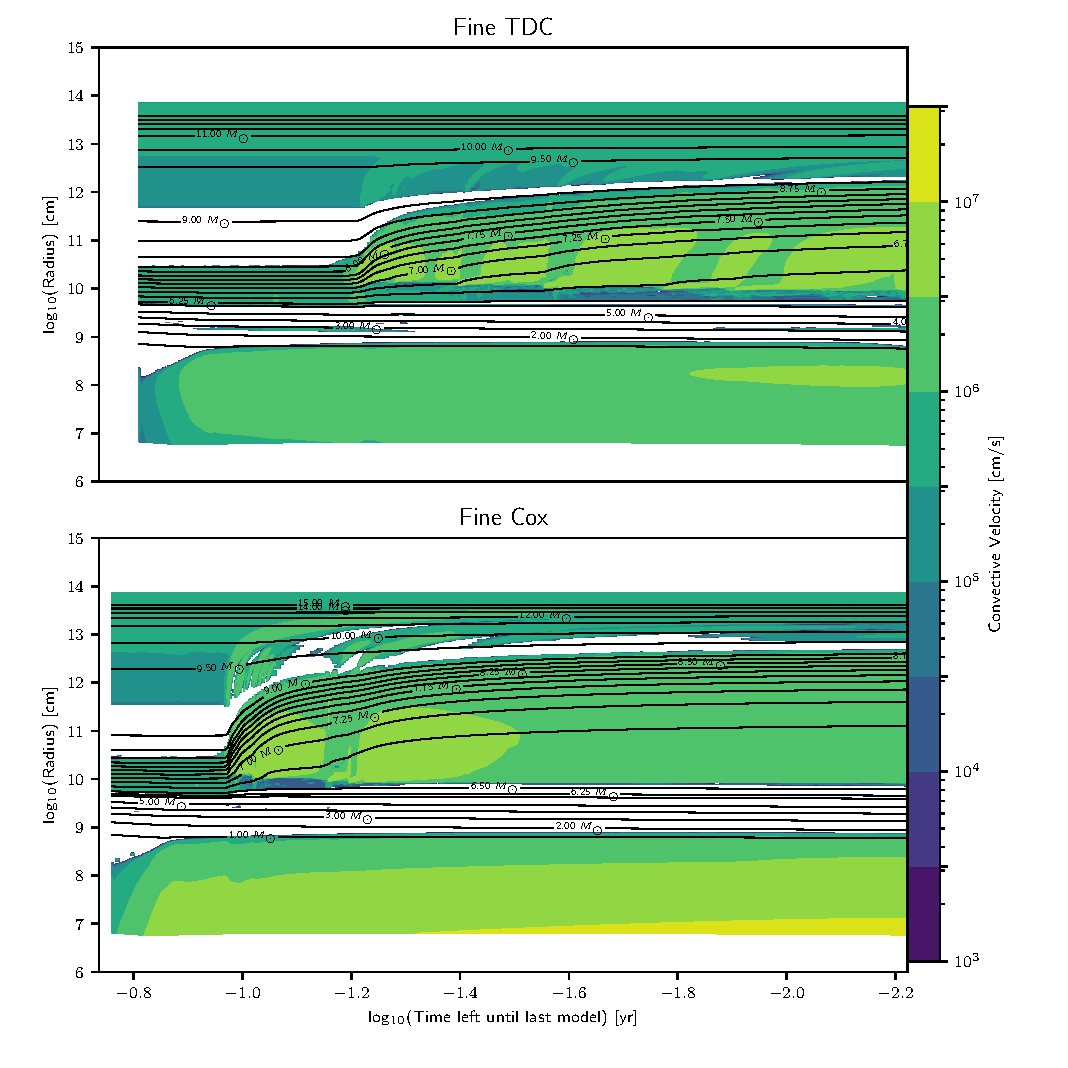
\includegraphics[width=\linewidth]{Figures/KHD_Compare_Mix.pdf}
%     \caption{Comparing an \gls{MLT} (lower) and \gls{TDC} (upper) run using short timestepping, focusing on a shell merger. Colour pertains to convective velocity.}
%     \label{fig:KHD_Compare_Mix}
% \end{subfigure}
% \hfill
% \begin{subfigure}{0.6\textwidth}
%     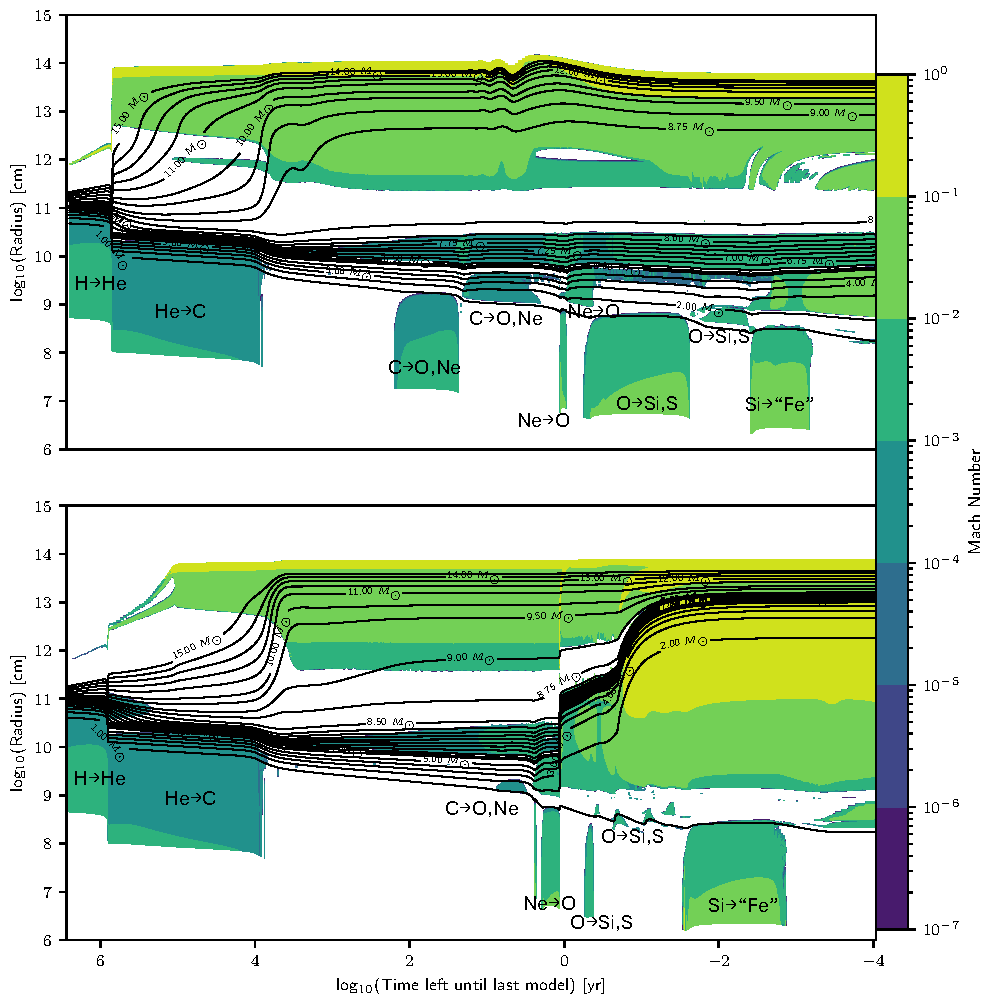
\includegraphics[width=\linewidth]{Figures/KHD_Compare_Metal.pdf}
%     \caption{Comparing a \gls{LowMetal} (lower) and \gls{SolarMetal} (upper) run using \gls{MLT} and short timestepping. Colour pertains to Mach number and label locations are based off of \citealp{Polls11}.}
%     \label{fig:KHD_Compare_Metal}
% \end{subfigure}
% \caption{Kippenhahn diagrams of radius (logarithmic) by time until core collapse.}
% \label{fig:KHDs}
% \end{figure*}